\documentclass[9pt]{sigplanconf}

\usepackage{amssymb}
\usepackage{amsmath}
\usepackage{amsthm}
\usepackage{stmaryrd}
\usepackage{color}
\usepackage{graphics}
\usepackage{fancyvrb}
\usepackage{subfigure}
\usepackage{amsthm}
\usepackage{tikz}
\usepackage{multirow}

\definecolor{darkblue}{rgb}{0.0,0.0,0.5}
\definecolor{darkgreen}{rgb}{0.0,0.4,0.0}

\usepackage[]{hyperref}
\hypersetup{
    unicode=false,          % non-Latin characters in Acrobat's bookmarks
    pdftoolbar=true,        % show Acrobat toolbar?
    pdfmenubar=true,        % show Acrobat menu?
    pdffitwindow=false,      % page fit to window when opened
    pdftitle={},    % title
    pdfauthor={}
    pdfsubject={},   % subject of the document
    pdfnewwindow=true,      % links in new window
    pdfkeywords={keywords}, % list of keywords
    colorlinks=true,       % false: boxed links; true: colored links
    linkcolor=darkblue,          % color of internal links
    citecolor=darkblue,        % color of links to bibliography
    filecolor=green,      % color of file links
    urlcolor=blue,          % color of external links
}


\CustomVerbatimEnvironment{SpecVerbatim}{Verbatim}{fontsize=\footnotesize,xleftmargin=0.5cm,
xrightmargin=0.2cm,commandchars=\\\{\},baselinestretch=0.98,numbersep=0.9em}
\CustomVerbatimEnvironment{ExmVerbatim}{Verbatim}{fontsize=\footnotesize,xleftmargin=0.5cm,
xrightmargin=0.2cm,baselinestretch=0.98,numbers=left,numbersep=0.9em}
\CustomVerbatimEnvironment{IVerbatim}{Verbatim}{fontsize=\relsize{-1},xleftmargin=0.5cm,
xrightmargin=0.2cm,commandchars=\\\{\},baselinestretch=0.98,numbersep=0.9em}


\definecolor{darkgreen}{rgb}{0.0,0.5,0.0}
\definecolor{darkpurple}{rgb}{0.6,0.0,0.6}
\definecolor{orange}{rgb}{0.8,0.4,0.0}
\definecolor{darkorange}{rgb}{0.5,0.2,0.0}
\definecolor{marco}{rgb}{0.0,0.3,0.5}
\definecolor{gray}{rgb}{0.2,0.2,0.2}

\newcommand{\bn}{\mathbb{N}}

\newcommand{\dnote}[1]{\textcolor{darkpurple}{Dom: #1}}
\newcommand{\mnote}[1]{\textcolor{darkgreen}{Mistral: #1}}

\newcounter{block}

\newtheorem{lemma}[block]{Lemma}
\newtheorem{proposition}[block]{Proposition}
%\newtheorem{definition}[block]{Definisssstion}

\theoremstyle{definition}

\newtheorem{theorem}[block]{Theorem}
\newtheorem{remark}[block]{Remark}
\newtheorem{example}[block]{Example}
\newtheorem{definition}[block]{Definition}

% Writing macros
\newcommand{\ie}{\emph{i.e.}}
\newcommand{\eg}{\emph{e.g.}}

\newcommand{\dimId}{\texttt{dim}}

% Semantics related
\newcommand{\interp}[1]{\llbracket{#1}\rrbracket}

% Syntax macros
\newcommand{\nonterm}[1]{\textit{#1}}
\newcommand{\term}[1]{\texttt{#1}}

\newcommand{\stenFwd}[2]{\term{forward} \, (\term{depth=}#1,
  \term{dim=}#2)}
\newcommand{\stenBwd}[2]{\term{backward} \, (\term{depth=}#1,
  \term{dim=}#2)}
\newcommand{\stenCen}[2]{\term{centered} \, (\term{depth=}#1,
  \term{dim=}#2)}
\newcommand{\stenFwdS}[2]{\term{fwd} \, (\term{depth=}#1,
  \term{dim=}#2)}
\newcommand{\stenBwdS}[2]{\term{bwd} \, (\term{depth=}#1,
  \term{dim=}#2)}
\newcommand{\stenCenS}[2]{\term{cen} \, (\term{depth=}#1,
  \term{dim=}#2)}


% SYNTAX OPERATIONS AND PREDICATES
\newcommand{\neigh}{\textsf{neigh}}
\newcommand{\arrayTy}{\textsf{array}}
\newcommand{\rhsExp}{\textsf{rhsExp}}
\newcommand{\var}{\textsf{var}}

%% VECTOR NOTATIONS
\newcommand{\vect}[1]{\textbf{#1}}
\newcommand{\vtwoh}[2]{\setlength{\arraycolsep}{0em}
\left[\begin{array}{cc}#1 \; & \; #2\end{array}\right]}
\newcommand{\vthreeh}[3]{\setlength{\arraycolsep}{0em}
\left[\begin{array}{ccc}#1 \; & \; #2 \; & \; #3\end{array}\right]}
\newcommand{\vtwo}[2]{\setlength{\arraycolsep}{0em}
\left[\begin{array}{l}$#1$\\$#2$\end{array}\right]}
\newcommand{\vthree}[3]{\setlength{\arraycolsep}{0em}
\left[\begin{array}{l}$#1$\\$#2$\\$#3$\end{array}\right]}
\newcommand{\stwo}[4]
%{\vtwo{#1}{#2}\!\vtwo{#3}{#4}}
{\setlength{\arraycolsep}{0.1em}
\left[\begin{array}{rr}$#1$ & $#3$\\$#2$ & $#4$\end{array}\right]}

\newcommand{\singleEntry}[2]{\textbf{J}_{#2}^{#1}}

%% OPERATIONS ON SPANS and VECTORS 
\newcommand{\containedin}{\sqsubseteq}


\title{Abstract Spatial Specification of Stencil Computations}
\authorinfo{Dominic Orchard \and Mistral Contrastin 
\and Matthew Danish \and Andrew Rice}{University of Cambridge}{}

\begin{document}
\maketitle

\begin{abstract}
  Verifying the correctness of numerical computations is hard because
  potential specifications for their behaviour tend to be highly
  decouple from the code, defined in terms of the originating
  mathematical model. For example, a system of PDEs specifies a
  relationship between variables, but tools for encoding such a
  specification, and pertinent properties such as convergence and
  stability, are rare.  Furthermore, checking the correctness of some
  implementation of a discrete approximation against such
  specifications is extremely challenging. We seek intermediate
  systems of specification and verification between lower-level
  aspects (\eg{}, out-of-bounds errors) and full correctness
  with-respect to a numerical model. In this paper, we focus on
  \emph{stencil computations}-- a common idiom in numerical code, but
  one which is prone to error due to fine-grained programming
  mistakes.  Our conjecture is that the vast majority of stencil
  computations have a simple, regular, static shape that can be
  described by a simple specification language. We propose a language
  for this, along with an inference and checking procedure. We test
  our conjecture against a corpus of numerical Fortran code, and show
  that static specifications can be given to $X\%$ of identifiable
  stencil computations, with a mean ratio of $Y:Z$
  specification-to-program code. This paper details our stencil
  specification language, its static semantics, inference, checking,
  and program synthesis procedures, our implementation, and our
  evaluation study.
\end{abstract}

\keywords{program verification, specifications, static analysis,
  stencil computation}

\bibliographystyle{abbrvnat}

\section{Introduction}

\emph{Stencils} are a ubiquitous programming pattern, common in
scientific and numerical computing applications. Informally, a stencil
computation computes an array value, where the value at each index $i$ of
this array is calculated from a \emph{neighbourhood} of values around $i$ in
some input array(s), \eg{}, the Game of Life, convolutions in image
processing, approximations to differential equations. For example, the
following iteratively computes the one-dimensional discrete Laplace
transform (an approximation to a derivative): 
%
\begin{ExmVerbatim}
do iter = 0, itermax
   do i = 1, (n-1)
      b(i) = a(i-1) - 2*a(i) + a(i+1)
   a = b
   end do
end do
\end{ExmVerbatim}
%
Line 3 is the core of the stencil computation, calculating
the value at \texttt{b(i)} from a neighbourhood of elements about
\texttt{a(i)}. Line 4 swaps
\texttt{a} and \texttt{b} between iterations, where \texttt{b} becomes the
input for the next iteration. Parentheses 
\texttt{( )} are used here for 
array subscripts rather than bracket syntax \texttt{[ ]}. 

%This stencil computation exhibits statically decideable
%spatial and temporal relationships between $\texttt{a}$ and
%$\texttt{b}$.
In this simple example, the dependency between \texttt{a}
and \texttt{b} on line 3 forms a simple spatial relationship which is easily
understood. This spatial relationship determines other aspects of the
program and its efficient implementation: how much ``boundary'' is
needed for the array, the most cache-efficient layout in memory,
the partitioning shape for parallel implementations. 

More complex stencil computations can be much harder to understand and
subsequently more prone to error. For example,
Figure~\ref{ref:navier-stokes-fragment} shows three lines from a
Navier-Stokes fluid simulator in which two arrays are read from with
different data access patterns, across two dimensions. The interaction
is much harder to understand, with the potential for the developer to
accidentally introduce an error via simple textual mistakes, for
example writing $\texttt{(i-1,j)}$ instead of $\texttt{(i+1,j)}$.

In this work, we introduce a simple specification language for the
spatial properties of stencil comptuations. The
specifications abstract over the fine grained detail of stencil access
patterns.  In practise, most stencil computations have a regular shape
that can be described simply and abstractly, with a small set of
coarse-grained descriptions. In the case of our first Laplace example,
our inference procedure provides the specification:
%
\begin{SpecVerbatim}
!=  stencil centered(depth=1, dim=1) :: a
\end{SpecVerbatim}
%
This explains that \texttt{a} is read from with a
symmetrical stencil pattern (``centered'') to a depth of one in each
direction in its first (and only) dimension.  
%The second line explains
%the temporal relationship between \texttt{b} and \texttt{a}: that
%previous time step for \texttt{b} is actually provided by \texttt{a},
%and vice versa. This is explained as a mutual dependence between
%\texttt{a} and \texttt{b}.
In the case of the Navier-Stokes example of
Figure~\ref{ref:navier-stokes-fragment}, its inferred specification is shown
in Figure~\ref{ref:navier-stokes-fragment}(b). The 
specification explains that, over the whole fragment, \texttt{u} is
read from with a centered pattern to depth of 1 in both dimensions
(this is known as the \emph{five point stencil}) and \texttt{v}
is read from in a neighbourhood bounded by forward to depth of $1$ in
the first dimension and backward to a depth of $1$ in the second
dimension. Figure~\ref{ref:navier-stokes-fragment}(c) describes these
pictorially. 

In this paper, we make the following contributions:
%
\begin{itemize}
\item we introduce a specification language for
stencil computations that captures many common forms
of data access pattern, both spatial and temporal (Section~\ref{sec:lang});
\item we detail inference and checking
algorithms for stencil specifications (Section~\ref{sec:analysis});
\item we evaluate our implementation of the approach
in the CamFort tool for Fortran verification, studying
a number of example programs to assess the usefulness
of this approach.
\dnote{insert results here}
\end{itemize}
%

\begin{figure}[t]
\begin{ExmVerbatim}[firstnumber=20]
du2dx = ((u(i,j)+u(i+1,j))*(u(i,j)+u(i+1,j))+
    gamma*abs(u(i,j)+u(i+1,j))*(u(i,j)-u(i+1,j))-
    (u(i-1,j)+u(i,j))*(u(i-1,j)+u(i,j))-
    gamma*abs(u(i-1,j)+u(i,j))*(u(i-1,j)-u(i,j)))
    /(4.0*delx)

duvdy = ((v(i,j)+v(i+1,j))*(u(i,j)+u(i,j+1))+
   gamma*abs(v(i,j)+v(i+1,j))*(u(i,j)-u(i,j+1))-
   (v(i,j-1)+v(i+1,j-1))*(u(i,j-1)+u(i,j))-
   gamma*abs(v(i,j-1)+v(i+1,j-1))*(u(i,j-1)-u(i,j)))
   /(4.0*dely)

laplu = (u(i+1,j)-2.0*u(i,j)+u(i-1,j))/delx/delx+
          (u(i,j+1)-2.0*u(i,j)+u(i,j-1))/dely/dely
\end{ExmVerbatim}
(a). Excerpt from Fortran code for a Navier-Stoke fluid simulator,
showing highly-detailed stencil computations. \\

%\begin{SpecVerbatim}[xleftmargin=0.1cm]
%20-24  u: centered depth=1 dim=1
%6-30  u: centered depth=1 dim=2
%      v: forward depth=1 dim=1, backward depth=1 dim=1
%32-33  u: centered depth=1 dim=1,2
%\end{SpecVerbatim}

\begin{SpecVerbatim}[xleftmargin=0.3cm]
!=   stencil centered(depth=1, dim=1)
           + centered(depth=1, dim=2) :: u

!=   stencil forward(depth=1, dim=1)
           * backward(depth=1, dim=2) :: v
\end{SpecVerbatim}
(b). Inferred stencil specification from CamFort

\begin{center}
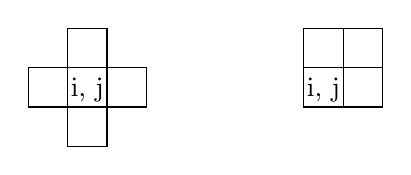
\begin{tikzpicture}
\node at (1.25,1.22) {i, j};
\draw (1,1) rectangle (1.5,1.5);
\draw (1.5,1) rectangle (2,1.5);
\draw (1,0.5) rectangle (1.5,1);
\draw (0.5,1) rectangle (1,1.5);
\draw (1,1.5) rectangle (1.5,2);
%
\node at (4.25,1.22) {i, j};
\draw (4,1) rectangle (4.5,1.5);
\draw (4.5,1) rectangle (5,1.5);
\draw (4.5,1.5) rectangle (5,2);
\draw (4,1.5) rectangle (4.5,2);
\end{tikzpicture}
\end{center}
(c). Pictoral representation of the two stencil specifications.
The horizontal dimensions is \text{dim=1} and the vertical is \texttt{dim=2}:
\caption{Fragment of Navier-Stokes fluid simulator and its specification}
\label{ref:navier-stokes-fragment}
\end{figure}

\section{Stencil specification language}
\label{sec:lang}

Our specification system is based on the observation
that most forms of array access in numberical code have
a fixed, statically-determined access pattern. For example, the
``\emph{five-point stencil}'' on a two-dimensional array reads from array
indices $(i, j)$, $(i-1, j)$, $(i+1, j)$, $(i, j-1)$, and $(i, j+1)$
for all $i, j$ within the inner boundary of the array (to avoid
out-of-bounds access at the edges). We revisit this hypothesis
in Section~\ref{sec:evaluation} where the inference of
such regular stencil patterns on a corpus of numerical programs (both
small and large). We found that indeed \dnote{..}.

We outline the specification language here. Section~\ref{sec:syntax}
oultines the syntax. Section~\ref{sec:semantics} defines its semantics
via a simple multi-set interpretation over indices. Section~\ref{sec:eqs} provides an
equational theory for specifications via relation ($\equiv$) and a
theory of approximation via relation ($<:$). These equations are then
proven sound with respecto the multi-set semantics of Section~\ref{sec:semantics}.

\subsection{Notation and convention}
\label{sec:notation}

\renewcommand*{\arraystretch}{0.8}
\paragraph{Target language syntax} Throughout, for the source language
syntax, $v$ ranges over program variables, $s$ over statements, and
$e$ over expressions (which may be impure).  By ``variable'', we mean
in the imperative sense (\ie{}, named binders to memory cells) instead
of mathematical variables. We make clear a number of standard notions
used throughout.

\begin{definition}[Base induction variable]
  An variable \textit{v} of integer type is a \emph{base induction
    variable} if it is the control variable of a ``for''
  loop\footnote{Or equivalent for the target language, \eg{},
    \texttt{do} in Fortan for our implementation}, incremented by $1$ per
iteration. The variable is marked as a base induction variable
only within the scope of the loop, and such variables will be ranged
over by $i$, $j$, $k$. Since we do not use non-base induction
variables (which are traditionally affine transformations of induction
variables) we often simply say \emph{induction variable}. 
\end{definition}

\begin{definition}[Array subscript]
  An \emph{array subscript} is an expression that indexes an array
  (for the purpose or reading or writing an element), which we denote
  by $v(\bar{e})$ for the source language where $\bar{e}$ is shorthand
  for a syntactic list of indexing expressions. A \emph{relative
    index} is a list $\bar{e}$ where each $e \in \bar{e}$ is defined
  in terms of some base induction variable.
\end{definition}

\begin{definition}[Neighbourhood index and neighbourhood subscripts]
  For an array subscript $v(\bar{e})$, we say say that $e \in \bar{e}$
  is a \emph{neighbourhood index} if it is of the form 
  $e \equiv i$, $e \equiv i + a$ or $e \equiv i - a$ where $a$ is a
  constant of integer type. That is, a neighbourhood index is a
  relative index defined as a constant translation of a base induction
  variable. The relation $\equiv$ identifies terms up-to commutativity
  of $+$ and the inverse relation of $+$ and $-$ (\eg{},
  $(-b) + i \equiv i - b$).  We classify neighbourhood indices using
  the predicate \neigh{}. An array subscript $v(\var{e})$ where every
 $e \in \bar{e}$ is a neighbourhood index is called a 
 \emph{neighbourhood subscript}. 
\end{definition}


\subsection{Specification syntax}
\label{sec:syntax}

Figure~\ref{fig:syntax} gives the syntax of stencil specifications,
which we introduces in stages below.  The top-level is given by the
\nonterm{specification} production which splits into either a
\nonterm{regionDec} (region declaration) or a \nonterm{specDec}
(specification declaration). Specification declarations associate a
specification to one or more program variables $\bar{v}$ (here given
using the Fortran style syntax of $\ldots \; \texttt{::} \bar{v}$),
describing how the array variables $\bar{v}$ are acessed.
%Specification declarations are either \nonterm{spatial} or
%\nonterm{temporal} specifications and describe, for spatial
%specifcations,
%Specifications declarations describe 
%how an array variable $v$ is read
%, and for temporal
%specifications what variables are used to define the array variable $v$.
%%

%\subsubsection{Spatial specification syntax}

\emph{Regions} are the central building blocks of spatial
specifications. Regions can either be declared along with a
\nonterm{regionDec}, assigning a region specification \nonterm{region} to
a region variable \nonterm{rvar} or given directly within a
\nonterm{spatial} specification.

\paragraph{Region constants}

Regions have as terminals the \emph{region constants}, denoted by 
\term{forward}, \term{backward}, or \term{centered}. Each
region constant is given a depth parameter $n$ (natural number greater
than 0) and a dimension identifier $d$ (also a natural number greater than
0). Region constants specify that an array is read from by a collection
of indices which in the $d^{th}$ dimension are 
neighbourhood indices ranging from $i + 0$ up to $i + n$ inclusively, \eg{}, the
following is valid stencil, reading from \term{a} and writing to \term{b}:
%%
\begin{ExmVerbatim}
!= stencil forward(depth=2, dim=1) :: a
b(i, 0) = a(i, 0) + a(i+1, 0) + a(i+2, 0)
\end{ExmVerbatim}
%%
were \texttt{i} is an induction variable.  The stencil specification
is associated to the array variable \texttt{a}. Note that the second
dimension is fixed at a constant here.

A \term{backward} stencil
is similar but has negative neighbourhood indices, \eg{}, 
%
\begin{ExmVerbatim}
!= stencil backward(depth=2, dim=1) :: a
b(i+1) = a(i) + a(i-1) + a(i-2)
\end{ExmVerbatim}
%
Note that the left-hand subscript on \term{b} does not affect
the stencil specification. The requirement on the left-hand side
is merely that it is an array subscript with at least one neighbourhood index,
but this may be on different induction variables to the right-hand
side, which is the stencil we are concerened with. 

A \texttt{centered} stencil is a combination of \texttt{forward}
and \texttt{backward} stencils to the same depth, \eg{},
%%
\begin{ExmVerbatim}
!= stencil centered(depth=1, dim=1) :: a
b(i) = ( a(i) + a(i-1) + a(i+1) ) / 3.0
\end{ExmVerbatim}

\begin{figure}[t]
\begin{align*}
\def\arraystretch{1.2}
\setlength{\arraycolsep}{0.2em}
\newcommand{\dimTy}{\mathbb{D}}
\begin{array}{rl}
\nonterm{specification} ::= & \nonterm{regionDec} \mid \nonterm{specDec} \\
\nonterm{specDec} ::= & \term{stencil} \; \nonterm{spec} \;
                        \texttt{::} \; v
  \\
\nonterm{regionDec} ::= &  \texttt{region} \; \nonterm{rvar} \; \texttt{=} \;
                         \nonterm{region}\\[1em]
%\nonterm{spec} ::= & \nonterm{spatial} \mid \nonterm{temporal}   \\[1em]
\nonterm{spec} ::= & [\nonterm{mod}] \;
                       [\nonterm{approxMod},] \; [\nonterm{region}] \\
\nonterm{mod} ::= & [\nonterm{modR},] \; [\nonterm{modRefl},] \; [\nonterm{modIrefl},] \\
\nonterm{modR} ::= &
 \term{readOnce} \\
\nonterm{modRefl} ::= & \term{reflexive} \, (\term{dims=}\dimTy \{\term{,} \; \dimTy\}) \\
\nonterm{modIrrefl} ::= & \term{irreflexive} \, (\term{dims=}\dimTy \{\term{,}
          \dimTy\}) \\
\nonterm{approxMod} ::= & \term{atMost} \; \mid \; \term{atLeast} \\[0.1em]
\nonterm{region} ::= & \stenFwd{\mathbb{N}_{>0}}{\dimTy}  \\
\mid \; & \stenBwd{\mathbb{N}_{>0}}{\dimTy} \\
\mid \; & \stenCen{\mathbb{N}_{>0}}{\dimTy} \\
\mid \; & \nonterm{region} \; \term{+} \; \nonterm{region} \\
\mid \; & \nonterm{region} \; \term{*} \; \nonterm{region} \\
\mid \; & \nonterm{rvar}  \\[0.5em]
%\nonterm{temporal} ::= \; & \term{dependency} \; (v \; \{ , v \}) [, \texttt{mutual}]
%  \\[0.5em]
\dimTy ::= \; & \mathbb{N}_{>0} \\
\nonterm{rvar} ::= \; & [\text{\term{a}-\term{z}$\,$\term{A}-\term{Z}$\,$\term{0}-\term{9}}]+
\end{array}
\end{align*}
\caption{Specification syntax (EBNF grammar)}
\label{fig:syntax}
\end{figure}

\paragraph{Sum and product of regions}
%%
Region terms can be combined using the sum operator
\term{+} or the product operator \term{*}. 

The sum of two regions $r \texttt{+} r'$ specifies that an array is
read using the neighbourhood indices described by both $r$ and
$r'$. It can be thought of as a conjunction of speicifcations. For
example, the following gives the specification for the five-point
stencil which is the sum of two \texttt{centered} regions in each
dimension:
%%
\begin{ExmVerbatim}
!= stencil centered(depth=1, dim=1) 
         + centered(depth=1, dim=2) :: a

b(i,j) = -4*a(i,j) + a(i-1,j) + a(i+1,j) 
                   + a(i,j-1) + a(i,j+1) 
\end{ExmVerbatim}
%%
The product of two regions $r \texttt{*} r'$ specifies that the array
is read with neighbourhood indices drawn from the bounding box created
by the regions two regions $r$ and $r'$. For example, the following
code (defining a nine-point stencil) has a specification as the
product of two \texttt{centered} regions in each dimension:
%%
\begin{ExmVerbatim}
!= stencil centered(depth=1, dim=1) 
         * centered(depth=1, dim=2) :: a

x = a(i, j)   + a(i-1, j)   + a(i+1, j)
y = a(i, j-1) + a(i-1, j-1) + a(i+1, j-1)
z = a(i, j+1) + a(i-1, j+1) + a(i+1, j+1)
b(i, j) = (x + y + z) / 9.0
\end{ExmVerbatim}
%%
Note that there are a number of intermediate assignments over which 
the whole specification ranges. 

\paragraph{Region declarations and variables}

Region specifications can be assigned to region variables via
a region declaration, which can be used later to form a spatial
specification. For example, the speicifcation from the previous
 example can be restated as:
%%
\begin{ExmVerbatim}
!= region r1 = centered(depth=1, dim=1) 
!= region r2 = centered(depth=1, dim=2)
!= stencil r1*r2 :: a
\end{ExmVerbatim}
%%
\paragraph{Spatial modifiers}
%%
There are three kinds of modifier that can be given to spatial 
specifications: \texttt{readOnce}, \texttt{reflexive}, 
\texttt{irreflexive}. 

The \texttt{readOnce} modifier enforces that no index appears
more than once. For example, in all of the previous examples the
\texttt{readOnce} modifier could be added, \eg{}
%
\begin{ExmVerbatim}
!= stencil readOnce, backward(depth=2, dim=1) :: a
b(i+1) = a(i) + a(i-1) + a(i-2)
\end{ExmVerbatim}
%
However, this would be an invalid specification if any of the 
array subscripts was reapeated. This modifier provides a way to
 rule out any accidental repetition of array subscripts. 
The notion correponds to that of \emph{linearity}, though we
opt for the more informative and easily understood name
\texttt{readOnce}. This modifier is optional, so it need not
be present even if the stencil is linear. 

The \texttt{irreflexive} modifier is parameteresed by a
comma-separated list of dimensions, indicating that for those
dimensions there is no neighbour index with $0$ offset, \eg{}, 
%
\begin{ExmVerbatim}
!= region r = centered(depth=1, dim=1)
!= stencil irreflexive(dim=1), r :: a
b(i) = a(i+1) + a(i-1)
\end{ExmVerbatim}
%
or with just a \texttt{forward} region an example would be: 
%
\begin{ExmVerbatim}
!= region r = forward(depth=1, dim=1)
!= stencil irreflexive(dim=1), r :: a
b(i) = a(i+1)
\end{ExmVerbatim}

The \term{reflexive} modifier is dual to \term{irreflexive},
indicating dimensions in which there is a neighbour index with $0$
offset. The region constants \term{forward}, \term{backward},
\term{centered} implicitly include the \term{reflexive} modifier,
but it is useful when there is a dimension in which there is reflexive
indexing but not a region constant, \eg{},
%%
\begin{ExmVerbatim}
!= region r = centered(depth=1, dim=1)
!= stencil reflexive(dims=2), r :: a
b(i,j) = a(i-1,j) + a(i+1,j) + a(i, j) 
\end{ExmVerbatim}
%%
Overlapping \term{irreflexive} and \term{reflexive} modifiers
cannot occur together-- this is an invalid specification.

\paragraph{Under and over-approximation}

In some cases, it is useful to give a lower and/or upper bound for a
stencil. This can be done using either the \term{atMost} or
\term{atLeast} modifiers. This is particularly useful in situations
where there is a non-contiguous stencil, which does not fit the rest
of the specification syntax.  For example:
%%
\begin{ExmVerbatim}
!= stencil atLeast, reflexive(dims=1)      :: a
!= stencil atMost, forward(depth=2, dim=1) :: a
b(i) = a(i) + a(i+2) 
\end{ExmVerbatim}
%%
%\subsubsection{Temporal specifications}


\subsection{Note on the design}

The names ``forward'', ``backward'' and ``centered''
are inspired by standard terminology in numerical analysis
for the shape of discretisation schemes. For example,
the standard ``explicit method'' for approximation
PDEs is the \emph{Forward Time, Centered Space} (FTCS)
scheme~\cite{dawson1991finite}. For
the one-dimensional heat equations, an FTCS discretisation 
provides approximation code with the following stencil~\cite{recktenwald2004finite}:
%%
\begin{ExmVerbatim}
do i=2:n-1
  u(i) = r*v(i-1) + r2*v(i) + r*v(i+1)
end do
\end{ExmVerbatim}
%%
where \texttt{r} and \texttt{r2} are some constants. 
A valid specification for this stencil is then:
%%
\begin{ExmVerbatim}
!= stencil centered(depth=1, dim=1) 
         + centered(depth=1, dim=2) :: v
\end{ExmVerbatim}
%%
Such a specification can be inferred, or can be inserted by a user
and checked against the code.

\subsection{Equational theory and approximations}
\label{sec:eqs}

\begin{figure}
\begin{align*}
\setlength{\arraycolsep}{0.05em}
\begin{array}{c}
\framebox{$\textit{region} \equiv \textit{region}'$} \\[1em]
\begin{array}{rll}
(\textsc{F\; \texttt{+} \;F}) \;\; &
\stenFwdS{n \, \textsf{max} \, m}{d} \\
 \equiv \; & \stenFwdS{n}{d} \; \texttt{+} \; \stenFwdS{m}{d} \\[1em]
%
(\textsc{B\; \texttt{+} \;B}) \;\; &
\stenBwdS{n \, \textsf{max} \, m}{d} \\
 \equiv \; & \stenBwdS{n}{d} \; \texttt{+} \; \stenBwdS{m}{d} \\[1em]
%
(\textsc{C\; \texttt{+} \;C}) \;\; &
\stenCenS{n \, \textsf{max} \, m}{d} \\
\equiv \; & \stenCenS{n}{d} \; \texttt{+} \; \stenCenS{m}{d} \\[1em]
%
(\textsc{C\; \texttt{+} \;F}) \;\; & \stenCenS{n}{d} \\
\textit{$m \leq n$} \; \equiv \; & \stenCenS{n}{d} \; \texttt{+} \;
                      \stenFwdS{m}{d} \\[1em]
%
(\textsc{C\; \texttt{+} \;B}) \;\; & 
\stenCenS{n}{d} \\
\textit{$m \leq n$} \; \equiv \; & \stenCenS{n}{d} \; \texttt{+} \;
                      \stenBwdS{m}{d} \\[1em]
(\textsc{B\; \texttt{+} \;F}) \;\; & 
\stenCenS{n}{d} \\
\equiv \; & \stenFwdS{n}{d} \; \texttt{+} \; \stenBwdS{n}{d} \\[1em]
%
(\texttt{+}\textsc{comm}) \;\; & S \; \texttt{+} \; T \; \equiv \; T \;
                       \texttt{+} \; S \\[0.5em]
%
(\texttt{+}\textsc{assoc}) \;\; & R \; \texttt{+} \; (S \; \texttt{+} \; T) \; \equiv \; (R \;
                       \texttt{+} \; S) \; \texttt{+} \; T \\[0.5em]
(\texttt{*}\textsc{comm}) \;\; & S \; \texttt{*} \; T \; \equiv \; T \;
                       \texttt{*} \; S \\[0.5em]
%
(\texttt{*}\textsc{assoc}) \;\; & R \; \texttt{*} \; (S \; \texttt{*} \; T) \; \equiv \; (R \;
                       \texttt{*} \; S) \; \texttt{*} \; T \\[0.5em] 
(\textsc{dist}) \;\; & R \; \texttt{*} \; (S \; \texttt{+} \; T) \; \equiv \; (R \;
                       \texttt{*} \; S) \; \texttt{+} \; (R
                       \; \texttt{*} \; T) \\[0.5em] 
(\textsc{inter}) \;\; & (S \; \texttt{+} \; S') \; \texttt{*} \;
                              (T \; \texttt{+} \; T') \\
 \equiv \; & (S \;  \texttt{*} \; S) 
 \; \texttt{+} \; (S \; \texttt{*} \; T') 
 \; \texttt{+} \; (S' \; \texttt{*} \; T)
 \; \texttt{+} \; (S' \; \texttt{*} T')  \\[0.5em] 
\end{array} \\ \\
%
\framebox{${\textit{specDec} :: \texttt{v}} \equiv 
{\textit{specDec'} :: \texttt{v}}$} \\[1em]
\begin{array}{rl}
% MUTUAL 
%(\textsc{mutual}) \; & 
%\texttt{stencil} \; \texttt{dependency} (\texttt{v}), \texttt{mutual}
%  :: \texttt{w} 
%\\
%\equiv \; & \texttt{stencil} \; \texttt{dependency} (\texttt{w}), \texttt{mutual} ::
%  \texttt{v} \\[0.5em]
%(\textsc{coalesce}) \; & 
%\texttt{stencil} \; \texttt{dependency} (\bar{v}) 
%  :: \texttt{v} \\
%& ; \texttt{stencil} \; \texttt{dependency} (\bar{w}) 
%  :: \texttt{v} 
%\\
%\equiv \; & \texttt{stencil} \; \texttt{dependency} (\bar{v}, \bar{w}) ::
%  \texttt{v} \\[0.5em]
(\textsc{spatial}) \; &
(\textit{region} \equiv \textit{region'}) \\
\Rightarrow \; & (\texttt{stencil} \; [\textit{mod}] \; [\textit{approxMod},] \;
\textit{region} \\
& \!\!\equiv \; \texttt{stencil} \; [\textit{mod}] \;
            [\textit{approxMod},] \;
\textit{region}') \\
\end{array}
\end{array}
\end{align*}
\caption{Equations on specifications}
\label{fig:equations}
\end{figure}


\paragraph{Equations}
Figure~\ref{fig:equations} lists the equational theory for
specifications. This is broken down into equations on regions only,
given by the equivalence relation $\textit{region} \equiv \textit{region}'$ and on
on specification declarations assigned to variables via the equivalence relation
$\textit{specDec} :: \texttt{v} \equiv
\textit{specDec'} :: \texttt{v}$.

To save space we use abbreviations 
\term{fwd}, \term{bwd}, and \term{cen} for \term{forward},
\term{backward}, and \term{centered} regions respectively.  The
equations reveal something of their semantics.  The first six
equations (with labels of the form $\ldots \texttt{+} \ldots$) 
explain the behaviour of overlapping regions with sum
\term{+}. The next six equations explain the algebraic behaviour of
\term{+} and \term{*}.  Together, we see that \term{+} is an
associative, commutative, idempotent binary operator that distributes
with \term{*}, which is associative and commutative. This distribution
of \term{*} over \term{+} is key as it is used internally to give a
normal form for stencil specifications akin to Disjunctive Normal Form
(DNF) (where \term{+} is taken as ``disjunction'' and \term{*} as the
``conjunction''). We revisit this normalisation in Section~\ref{}.

\begin{figure}[t]
\begin{align*}
\begin{array}{c}
\dfrac{}{S <: S}(\textsc{refl}) \qquad \dfrac{R <: S \quad S <: T}{R <:
  T}(\textsc{trans}) \\[1.5em]
\dfrac{}{\texttt{readOnce} \, S <: S}(\textsc{rep})
\\[1.5em]
\setlength{\arraycolsep}{0.1em}
\dfrac{\hspace{3em} m \leq n \hspace{3em}}
{\begin{array}{rl}
\stenFwdS{m}{d} & <: \stenFwdS{n}{d}
%& \;\, ds \subseteq es \wedge n \leq m
\\
\wedge \stenBwdS{m}{d} & <: \stenBwdS{n}{d}
%& \;\, ds \subseteq es \wedge n \leq m
\\
\wedge \; \stenCenS{m}{d} & <: \stenCenS{n}{d}
%& \;\, ds \subseteq es \wedge n \leq m
\\
\wedge \; \stenBwdS{m}{d} & <: \stenCenS{n}{d} \\
\wedge \; \stenFwdS{m}{d} & <: \stenCenS{n}{d} \\[1em]
\end{array}} \\[2.5em]
\hspace{-0.5em}
\dfrac{S_1 <: T_1 \quad S_2 <: T_2} 
      {S_1 \, \texttt{+} \, S_2 <: T_1 \, \texttt{+} \, T_2}
(\textsc{cong}\texttt{+}) \;\;\;
\dfrac{S_1 <: T_1 \quad S_2 <: T_2} 
      {S_1 \, \texttt{*} \, S_2 <: T_1 \, \texttt{*} \, T_2}
(\textsc{cong}\texttt{*})
\end{array}
\end{align*}
\caption{Inequations on regions}
\label{fig:inequations}
\end{figure}

\paragraph{Inequations: sub-specifications}

Figure~\ref{fig:inequations} 

\section{Semantics of specifications; a model}
\label{sec:semantics}

\newcommand{\relix}{(\mathbb{Z}_\bot)^\mathbb{D}}

We provide a semantic model of the stencil specification language as
the basis for building correct implementations, showing the soundness
of the equational theory and approximations, and as a basis for the
inference, checking, and program synthesis algorithms.
The semantics of stencil specifications can be given a denotational
model as multisets of vectors, represent array indexing.

\begin{definition}
  A specification of maximum dimensionality $n$, is modelled by a
  multi-set of column vectors of size $n$  ($n$-dimensional vectors /
  $n$-vectors for short)
  with values drawn from $\mathbb{Z} \cup \{\infty\}$, representing
  relative indices. The $\infty$ element represents non-relative
  indices (\eg{}, constants), which are seen as infinite with respect
  to the frame of reference of a relative offset from an induction
  variable.

  For example, the array index $(i, j+1)$ corresponds to the vector
  $\vtwoh{0}{1}$, whereas, the $(0, j)$ corresponds to the
  vector $\vtwoh{\infty}{0}$ since $0$ is a non-relative index. 
\end{definition}
 
Figure~\ref{fig:model} outlines the core rules for regions
via the interpretation function $\interp{-}$.  We explain the
intermediate notations and definitions:

\begin{definition}A \emph{single-entry vector} of size $n$, denoted 
$\singleEntry{r}{n}$, is a vector 
where the $r^{th}$ entry is $1$ and all others are $0$, \eg{},
$\singleEntry{1}{2} = \vtwoh{1}{0}$.
\end{definition}

\begin{definition}The product of two models $\otimes$ is defined:
%%
\begin{align*}
M \otimes N & =
  \{(u \bowtie v)_i \mid i \in \{0, \ldots, 2^n \}, (u, v) \in
              M \times N\}^1
\end{align*}
The $\bowtie$ operation, which we call \emph{pairwise permutation}
(described below), constructs a $2^n \times n$ matrix ($2^n$-vector of
$n$-vectors).  Using this, the $\otimes$ operation constructs the set
of every pairwise permutation for every pair $(u, v)$ of $n$-vectors in the
Cartesian product of $M \times N$. Note the $^1$ superscript here 
on the set-builder notation which denotes that this construction
constructs a degenerate multiset (where all the multiplicities are 1).
This is important for the function of $\otimes$ in the model (see below).

The pairwise permutation $u \bowtie v$ takes two vectors and builds the matrix
where the rows are all possible $n$-vectors generated by 
non-determinstically picking each $i^{th}$ entry from either the
$i^{th}$ entry in $u$ or the $i^{th}$ entry in $j$. For example:  
%
\begin{equation*}
\vthreeh{0}{1}{2} \bowtie \vthreeh{3}{4}{5} = 
\setlength{\arraycolsep}{0.5em}
\left[\begin{array}{ccc}
0 & 1 & 2 \\
0 & 1 & 5 \\
0 & 4 & 2 \\
0 & 4 & 5 \\
3 & 1 & 2 \\
3 & 1 & 5 \\
3 & 4 & 2 \\
3 & 4 & 5 
\end{array}
\right]
\end{equation*}
%
The $2^n$ unique choices for $\bowtie$ on $n$-vectors 
corresponds to taking all bit-strings of length $n$ and
selecting from $u$ for $1$ and $v$ for $0$. Thus, we can
defined the pairwise pemutation matrix as:
%
\begin{align*}
(u \bowtie v)_{i,j} & = b_{i,j} u_i + \neg b_{i,j} v_i
\end{align*}
%
where $b$ is a logical matrix where $b_{i,j}$ is the $j$-th bit of the integer $i$. 
Recall that the vectors are defined over the domain
$\mathbb{Z} \cup \{\infty\}$. 
For addition and multiplication, we take 
 $\infty$ to be an absorbing element. Thus, if either
vector in a pairwise permutation contains $\infty$ in
the $j^{th}$ entry, then $j^{th}$ entry of every pairwise
permutation is $\infty$, \eg{}, 
%%
\begin{equation*}
\vtwoh{0}{1} \bowtie \vtwoh{2}{\infty} = 
\setlength{\arraycolsep}{0.5em}
\left[\begin{array}{cc}
0 & \infty \\
0 & \infty \\ 
2 & \infty \\
2 & \infty
\end{array}
\right]
\end{equation*}


%%
\end{definition}


%The main interpretation function is overloaded on lists of
%variable-spec pairs $\interp{\overline{v : S}}$,
%returning multisets of variable-relative-index pairs. This provides
%the top-level definition of the model, with $\interp{-}$ overloaded
%on $S$, $\interp{S}$ mqpping to multisets of
%relative indices not associated to an array avariable.

\begin{figure}
\newcommand{\singleEntry}[2]{\textbf{J}_{#2}^{#1}}
\begin{align*}
%
% REGION model
%
\interp{\stenFwd{k}{d}}^r_n & =
 \{i\singleEntry{d}{n} \mid i \in \{0, \ldots, k\} \} \\
\interp{\stenBwd{k}{d}}^r_n & =
 \{i\singleEntry{d}{n} \mid i \in \{-k, \ldots, 0\} \} \\
\interp{\stenCen{k}{d}}^r_n & =
 \{i\singleEntry{d}{n} \mid i \in \{-k, \ldots, k\} \} \\
%
% REGION PROD model
%
\interp{r_1 \; \texttt{$\ast$} \, \ldots \, \texttt{$\ast$} \; r_m}^{\ast}_n &
= \interp{r_1}^r_n \otimes \ldots \otimes \interp{r_m}^r_n \\
%
%  REGION SUM model
%
\interp{r_1 \; \texttt{+} \, \ldots \, \texttt{+} \; r_m}^{+}_n &
= \interp{r_1}^{\ast}_n \cup \ldots \cup \interp{r_m}^{\ast}_n \\
\end{align*}
%where $\singleEntry
TODO: insert explanation for the $\textbf{J}$ notation (see Matrix
textbook).


%\textit{$a^m \in A$ means there are $n$ copies of $a$ in
%  the multi-set $A$}
\caption{Multi-set model of specifications}
\label{fig:model}
\end{figure}

\begin{theorem}[Soundness]
\[
\overline{\texttt{v} : S}\equiv \overline{\texttt{u} : T}
\; \Rightarrow \;
\interp{\overline{\texttt{v} : S}} = \interp{\overline{\texttt{u} : T}}
\]
\end{theorem}

\paragraph{Proof} (see Appendix)

\begin{theorem}[Soundness]
\[
\overline{\texttt{v} : S} <: \overline{\texttt{u} : T}
\; \Rightarrow \;
\interp{\overline{\texttt{v} : S}} \subseteq \interp{\overline{\texttt{u} : T}}
\]
\end{theorem}

\paragraph{Proof} (see Appendix)



\section{Inference, checking, and synthesis}
\label{sec:analysis}

\mnote{Few cases that we might like to consider (there are examples
    of each in \#camfort-main Slack channel):
  \begin{itemize}
    \item Matrix operator overloading $a + b$, where both are arrays
    \item Scalar operator overloading $a + b$, where a is an array b is a
      scalar. $b$ is added to all.
    \item Sliding. $a = b$ where the dimensionsare $a(1:10)$, $b(2:11)$,
      so the assignment causes shifting.
  \end{itemize}
}

\noindent
We briefly sketch the algorithms for inferring and checking
specifications and for synthesising programs from specifications.
Checking and synthesis use the set-based semantic model of
Section~\ref{sec:semantics}. 

\paragraph{Syntax functions}
The function \rhsExp{} maps statements to a
set of expressions which occur in right-hand positions (\ie{}, not the
target of an assignment). The function \var{} maps expressions to a
set of the variables used in right-hand positions.

\subsection{Inference}

We demonstate the main steps of the inference procedure over the
following example program which computes the mean value 
of a five-point stencil at each index of the input array:
%%
\begin{ExmVerbatim}
do i = 1, (n-1)
   do j = 1, (m-1)
      x       = a(i-1, j) + a(i+1, j) 
      y       = a(i, j-1) + a(i, j+1)
      b(i, j) = (a(i, j) + x + y) / 5.0
   end do
end do
\end{ExmVerbatim}
%%
\paragraph{Step 1: Standard control and dataflow analyses}
The inference relies on some standard program analyses, computed
before the main inference procedure:
%
\begin{enumerate}
\item basic blocks (CFG);
\item induction variables per basic block;
\item (interprocedural) dataflow analysis, providing a \emph{flows to}
  graph (as shorthand, the function
  $\mathsf{flowTo}$ is used, implicitly parameterised by this graph,  
  mapping an expression to the set of all expressions
  with forwards dataflow to this expression, based on the transitive
  closure of the flows graph);
\item type information per variable, where we use the predicate
\arrayTy{} to classify variables of array type. 
\end{enumerate}
%

\paragraph{Step 2: Data-access analysis}

For each assignment statement whose left-hand side is an array
subscript on neighbourhood indices, a finite map is computed which
maps array variables to a set of vectors representing array
subscripts.  This finite map contains all array subscript expressions
which flow to this statment. More formally, a function
$\textsf{analyse}$ is applied to each statement in a program with the
following clause:
%
\begin{align*}
\begin{array}{lr}
\textsf{analyse}(v(\overline{e_1}) = e_2)
 := \qquad\qquad & \textit{where} \; \neigh(\overline{e_1}) \wedge \arrayTy(v)  \\[0.3em]
\multicolumn{2}{l}{\qquad \bigcup\{v' \mapsto \{\textsf{convert}(\bar{e})\} \mid v'(\bar{e}) \leftarrow \mathsf{flowsTo}(e_2),
  \arrayTy(v')\}}
\end{array}
\end{align*}
%
That is, we focus on assignments to an array subscript where each
index indexing expression in $\bar{e}$ is a neighbourhood index.  For
all array subscripts that flow to the right-hand side of this
statement, a finite map is constructed from each array variable
in this flow set to a representation of the subscripts, computed
with \textsf{convert}.

The \textsf{convert} function maps subscripts to a column vector
representation with values drawn from $\mathbb{Z}_\top = \mathbb{Z} \cup \{\top\}$
where $\mathbb{Z}$ represents the offset of a neighbourhood index
and $\top$ represents any non-neighbourhood subscripts, defined:
%
\begin{align*}
& \textsf{convert}((e_1, \ldots, e_n)) = [\textsf{conv}(e_1), \ldots,
  \textsf{conv}(e_n)] \\
& \textsf{conv}(e) \begin{cases}
\pm a & \neigh(e) \wedge \, e \equiv i \pm a \\
\top & \textit{otherwise} 
\end{cases} 
\end{align*}
%
For our example, the \textsf{analyse} function matches on
line 5, with the following set for $\textsf{flowTo}(a(i, j) + x +
  y)$:
%
\begin{align*}
\{\texttt{a(i-1, j)}, \texttt{a(i+1, j)}, \texttt{a(i, j-1)},
  \texttt{a(i, j+1)}, \texttt{a(i, j)}\}
\end{align*}
Subsequently the result of \textsf{analyse} on line 5 yields the map:
\begin{align*}
\texttt{a} \mapsto \{\vtwo{-1}{0}, \vtwo{1}{0},
          \vtwo{0}{-1}, \vtwo{0}{1}, \vtwo{0}{0}\}
\end{align*}
%

\paragraph{Step 3: Coalesce contiguous indices into regions}

Let $M$ range over the finite maps generated by \textsf{analyse}.  For
each $v \in \mathsf{dom}(M)$, the algorithm then constructs a group
of regions which cover all contiguous groups of relative indices
(from $M(v)$) in the $n$-dimensional space. 

Informally, the procedure proceeds as follows. First, relative
indices are turned into unit regions in $n$-dimensions. For
example, for the five point stencil there are five $1 \times 1$ regions,
called \emph{spans}, which are essentially $0$-dimensional:
%
\begin{center}
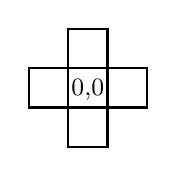
\begin{tikzpicture}
%\draw[step=0.5cm,lightgray,very thin] (0.5,0.5) grid (2,2);
\node at (1.25,1.22) {\textnormal{\small{0,0}}};
\draw[thick] (1,1) rectangle (1.5,1.5);
\draw[thick] (1.5,1) rectangle (2,1.5);
\draw[thick] (1,0.5) rectangle (1.5,1);
\draw[thick] (0.5,1) rectangle (1,1.5);
\draw[thick] (1,1.5) rectangle (1.5,2);
\end{tikzpicture}
\end{center}
%
Each dimension is traversed, coalescing consecutive spans
which vary in $m$-dimensions into coalesced spans which vary in 
$m+1$-dimensions. In this example, the $0$-dimensional spans
 become $1$-dimensional spans (rows/columns):
%
\begin{align*}
\begin{array}{cc}
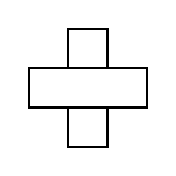
\begin{tikzpicture}
%\draw[step=0.5cm,lightgray,very thin] (0.5,0.5) grid (2,2);
%\node at (1.25,1.22) {\textnormal{\small{0,0}}};
\draw[thick] (0.5,1) rectangle (2,1.5);
\draw[thick] (1,0.5) rectangle (1.5,1);
\draw[thick] (1,1.5) rectangle (1.5,2);
\end{tikzpicture}
\qquad
&
\qquad
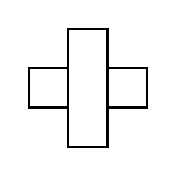
\begin{tikzpicture}
%\draw[step=0.5cm,lightgray,very thin] (0.5,0.5) grid (2,2);
%\node at (1.25,1.22) {\textnormal{\small{0,0}}};
\draw[thick] (1.5,1) rectangle (2,1.5);
\draw[thick] (0.5,1) rectangle (1,1.5);
\draw[thick] (1,0.5) rectangle (1.5,2);
\end{tikzpicture}
\\
\textit{dimension 1} \qquad & \qquad \textit{dimension 2}
\end{array}
\end{align*}
%
Any spans that are contained with any other span are deleted,
leaving a minimal set of spans (which may overlap, but none of which
fully contains another).
\begin{center}
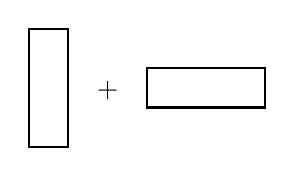
\begin{tikzpicture}
%\node at (1.25,1.22) {\textnormal{\small{0,0}}};
\draw[thick] (1,0.5) rectangle (1.5,2);
\node at (2,1.22) {+};
\draw[thick] (2.5,1) rectangle (4,1.5);
%\node at (2.75,1.22) {\textnormal{\small{0,0}}};
\end{tikzpicture}
\end{center}
%
The procedure is then iterated till a fixed point is reached. In this
example this is reached in the first step. These final spans
go on to form the basis of the spatial stencil specification, where
each span is a region product \texttt{*} and multiple spans are
combined with the region sum \texttt{+}.


\paragraph{Span coalescing, formally}

Let $\vect{x}, \vect{y}, \vect{z}$ range over the column vectors of size
$n$ whose values are drawn from $\mathbb{Z}_\top$.
We write $\vect{x}_i$ for the $i$-th value of vector $\vect{x}$ (1
indexed) and $\vect{x}_{i:j}$ for the subvector from entry $i$ to
entry $j$ (inclusive). 

\begin{definition}[Spans]
  A \emph{span} represents an $n$-dimensional box (\emph{hyperrectangle}) as
  a pair of $n$-dimensional vectors (represented as a $2 \times n$
  matrix) giving the co-ordinates of the lower-bound vertex (first
  column) and the upper-bound vertex (second column). We use the
  notation $[\vect{x}^L \; \vect{x}^U]$ for such a span to mark out
  the lower and upper bound vecvtors. 
\end{definition}

The algorithm to create contiguous spans, covering the space of
indices, then proceeds as follows. 
Firstly, for all $v \in \mathsf{dom}(M)$ then a new map $M'$ is
created where each vector is mapped to the trivial \emph{unit span} is
created by pairing a vector with itself:
%
\begin{align*}
N(v) = \{[\vect{x} \; 
  \vect{x}] \mid \vect{x} \in M(v)\}
\end{align*}
%
For our example, this yields:
%%
\begin{align*}
N(\texttt{a}) = \stwo{0}{0}{0}{0} \stwo{1}{0}{1}{0} \stwo{-1}{0}{-1}{0} \stwo{0}{1}{0}{1} \stwo{0}{-1}{0}{-1}
\end{align*}
%%
A fixed point is then compute for the following
procedure \textsf{regions} which, for per variable
in the map, coalesces spans into contiguous regions in
the $n$-dimensional spaace. That is, we compute
 $(\mu \; \textsf{regions}) N$ where \textsf{regions}
is defined as follows for each variable in the map:
%
\begin{enumerate}

\item Compute all permutations on the column vectors in a span, \ie{},
  $[\vect{x}^L \vect{x}^U] \mapsto [\pi\vect{x}^L \, \pi\vect{x}^U]$
for a permutation $\pi$. For each permutation function $\pi^n_i$
(the $i$-th permutation for vectors of size $n$, we pair the
permutation function with the set of permuted spans so that 
the spans can be unpermuted later. 
%
\[
P(v) = \bigcup_{i \in !n} (\pi^n_{i} , \; \{[\pi^n_i
\vect{x}^L \; \pi^n_i\vect{x}^U] \, \mid \, [\vect{x}^L \; \vect{x}^U]
\leftarrow N(v)\}
\]
%
For our example, this yields:
%
\begin{align*}
P(\texttt{a}) = 
\{&(\pi^2_1, \{ \stwo{0}{0}{0}{0}
\stwo{1}{0}{1}{0} 
\stwo{-1}{0}{-1}{0} 
\stwo{0}{1}{0}{1} 
\stwo{0}{-1}{0}{-1} \})
\\
&(\pi^2_2, \{ 
 \stwo{0}{0}{0}{0}
 \stwo{0}{1}{0}{1}
 \stwo{0}{-1}{0}{-1}
 \stwo{1}{0}{1}{0}
 \stwo{-1}{0}{-1}{0}\})\}
\end{align*}
%
where $\pi^2_1$ is the identity permutation and $\pi^2_2$ is the
permutation flips the order of the two elements in the column
vectors. 

\item Sort each permutation set into an ordered list, based on the ordering:
\[
\vect{x} \leq \vect{y} = \exists i \, . \; \vect{x}_i \leq \vect{y}_i 
\; \wedge \; \vect{x}_{i:n} = \vect{y}_{i:n}
\]
%
This yields:
%%
\begin{align*}
\{&(\pi^2_1, [
\stwo{0}{-1}{0}{-1}
\stwo{-1}{0}{-1}{0} 
\stwo{0}{0}{0}{0}
\stwo{1}{0}{1}{0} 
\stwo{0}{1}{0}{1}] )
\\
&(\pi^2_2, [
\stwo{0}{-1}{0}{-1}
\stwo{-1}{0}{-1}{0}
\stwo{0}{0}{0}{0}
\stwo{1}{0}{1}{0}
\stwo{0}{1}{0}{1}])\}
\end{align*}
%%
\item Fold each list pairwise by the following partial operation
 $\bullet$ which coalescees contiguous regions:
%
\begin{align*}
& (\vect{x}^L,\vect{x}^U) \bullet (\vect{y}^L,\vect{y}^U) \\
= &
\begin{cases}
(\vect{x}^L, \vect{y}^U) & \vect{x}^U_1 + 1 = \vect{y}^L_1 \; \wedge \;
(\vect{x}^L_{1:n}, \vect{x}^U_{1:n}) = (\vect{y}^L_{1:n}, \vect{y}^U_{1:n}) \\
\bot  & \textit{otherwise}
\end{cases}
\end{align*}
For our example, this yields:
%
\begin{align*}
Q(v) = \{&(\pi^2_1, [
\stwo{0}{-1}{0}{-1}
\stwo{-1}{0}{1}{0}, 
\stwo{0}{1}{0}{1}, 
]) \\
&(\pi^2_2, [
\stwo{0}{-1}{0}{-1},
\stwo{-1}{0}{1}{0},
\stwo{0}{1}{0}{1}])\}
\end{align*}
%
\item Unpermute and union together, \ie{},
%
\[
U(v) = \bigcup \{[\pi \vect{y}^L, \pi \vect{y}^U]
 \mid [\vect{y}^L, \vect{y}^U] \leftarrow S, (\pi, S) \leftarrow Q(v)\}
\]
Which yields:
%
\begin{align*}
U(\texttt{a}) = 
\{\stwo{0}{-1}{0}{-1}
\stwo{-1}{0}{1}{0}
\stwo{0}{1}{0}{1}
\stwo{-1}{0}{-1}{0}
\stwo{0}{-1}{0}{1}
\stwo{1}{0}{1}{0}\}
\end{align*}
%
\item Finally, filter by the region containment predicate $\containedin$, that
  is, if any region is contained within another then remove the
  smaller. The $\containedin$ predicate is defined:
%
\begin{align*}
& (\vect{x}^L, \vect{x}^U) \containedin (\vect{y}^L, \vect{y}^U) = \\
& \vect{y}^L_1 \leq \vect{x}^L_1 \wedge \vect{x}^U_1 \leq \vect{y}^U_1
  \wedge (\vect{x}^L_{1:n}, \vect{x}^U_{1:n}) \containedin
  (\vect{y}^L_{1:n}, \vect{y}^U_{1:n})
\end{align*}
For our example this then yields the final result of: 
\begin{align*}
\textsf{regions}(M) 
= \{\stwo{-1}{0}{1}{0} \stwo{0}{-1}{0}{1}\}
\end{align*}
since $\stwo{0}{1}{0}{1} \sqsubseteq \stwo{0}{-1}{0}{1}$
and $\stwo{1}{0}{1}{0} \sqsubseteq \stwo{-1}{0}{1}{0}$. 
\end{enumerate}
For our example, applying \textsf{regions} again yields the same
result, hence we have reached a fixed point.

\paragraph{Step 4: Convert spans into region AST}

Given the set $\textsf{regions}(M)$ of spans covering the indexing
space, the next step converts these into abstract syntax tree
for the specification language.


\section{Evaluation}
\label{sec:evaluation}

\section{Discussion}
\label{sec:discussion}


\bibliography{references}


\onecolumn
\appendix

\section{Correctness}


\begin{theorem}[Soundness]
\[
\overline{\texttt{v} : S}\equiv \overline{\texttt{u} : T}
\; \Rightarrow \;
\interp{\overline{\texttt{v} : S}} = \interp{\overline{\texttt{u} : T}}
\]
\end{theorem}

\paragraph{Proof}
\begin{itemize}
\item \textsc{coalesceF}
\begin{align*}
\llbracket & \texttt{v} : \texttt{fwd} \; \texttt{dims}=ds \; \texttt{depth}=n; \,
  \texttt{v} :  \texttt{fwd} \; \texttt{dims}=ds \;
  \texttt{depth}=n+1)\rrbracket \\
& =  \{ (\texttt{v}, ix)^m \mid \forall \, m, ix : \relix, d : \mathbb{N}
  \, . \, d \in \textit{ds} \Rightarrow ix \, d \leq (n+1) \} \; \cup \; \{ ix^m \mid \forall \, m, ix : \mathbb{Z}^{\mathbb{N}}, d : \mathbb{N}
  \, . \, d \in \textit{ds} \Rightarrow ix \, d \leq n \}\\
& =  \{ (\texttt{v}, ix)^m \mid \forall \, m, ix : \relix, d : \mathbb{N}
  \, . \, d \in \textit{ds} \Rightarrow ((ix \, d \leq (n+1)) \vee (ix \,
  d \leq n)) \} \\
& =  \{ (\texttt{v}, ix)^m \mid \forall \, m, ix : \relix, d : \mathbb{N}
  \, . \, d \in \textit{ds} \Rightarrow ix \, d \leq (n+1) \} \\
& = \interp{\texttt{v} : \texttt{fwd} \; \texttt{dim}=ds \;
  \texttt{depth}=n + 1} \qquad \Box
\end{align*}
\end{itemize}

\end{document}
